\chapter{RESULTADOS EXPERIMENTALES} \label{chap:resultados}

Este capítulo presenta los resultados obtenidos de la implementación y evaluación de los 
modelos de clasificación de retinopatía diabética desarrollados, se organiza en dos secciones principales: 
primero se presentan los resultados de la clasificación binaria (presencia/ausencia de 
RD), incluyendo la comparación de arquitecturas CNN, el impacto del preprocesamiento 
mediante filtrado, la optimización del umbral de decisión, el análisis estadístico 
mediante bootstrap y la validación externa en tres datasets independientes. 
Posteriormente se exponen los resultados de la clasificación multiclase (gradación en 
cinco niveles de severidad), con énfasis en el análisis comparativo del desempeño al 
procesar diferentes canales de color (RGB, rojo, verde, azul).

\section{CLASIFICACIÓN BINARIA}

\subsection{Comparación de arquitecturas CNN preentrenadas}

Se implementó una estrategia de aprendizaje por transferencia utilizando diversas redes 
preentrenadas disponibles en Keras Applications. Debido a que cada red requiere un tamaño 
de entrada específico, se seleccionaron finalmente VGG19, ResNet50V2, InceptionV3 y 
MobileNetV2, todas con tamaños de entrada compatibles ($224 \times 224$ píxeles). Estas 
arquitecturas permiten analizar la estrategia tanto desde el punto de vista de desempeño 
como de eficiencia computacional, considerando la velocidad de inferencia y la cantidad 
de parámetros. Además, se eligieron para comparar el comportamiento de redes clásicas, 
como VGG19, frente a arquitecturas más modernas, como MobileNetV2.

En la Tabla~\ref{tab:comparacion_redes} se presentan los resultados obtenidos al entrenar
el modelo CNN variando entre estas redes preentrenadas, fijando un umbral de decisión de
0.5, con el objetivo de identificar la red base con mejor desempeño en la clasificación
binaria en términos de precisión, sensibilidad, F1-score y especificidad. Dado que RD se
define como la clase positiva y No RD como la clase negativa, la sensibilidad (recall de
RD) y la especificidad (recall de No RD) ya tienen una interpretación única respecto a
esa definición; por ello, a diferencia de un reporte de métricas por clase, se presenta
una sola fila por arquitectura en lugar de repetir ambas métricas para cada clase.

\begin{table}[ht!]
	\centering
	\renewcommand{\arraystretch}{1.2}
	\caption{Desempeño de redes preentrenadas para clasificación binaria de
retinopatía diabética usando el dataset original de Kaggle (RD como clase positiva)}
	\label{tab:comparacion_redes}
	\begin{tabularx}{\textwidth}{l Y Y Y Y}
		\toprule
		Red Preentrenada & Sensibilidad & Especificidad & Precisión & F1-score \\
		\midrule
		MobileNetV2 & \textbf{0.95} & \textbf{0.94} & \textbf{0.95} & \textbf{0.95} \\
		ResNet50V2 & 0.77 & 0.78 & 0.77 & 0.77 \\
		InceptionV3 & 0.71 & 0.72 & 0.71 & 0.71 \\
		VGG19 & 0.86 & 0.85 & 0.86 & 0.86 \\
		\bottomrule
	\end{tabularx}
	\caption*{\textit{Fuente: Elaboración propia}}
\end{table}

Según la Tabla~\ref{tab:comparacion_redes}, MobileNetV2 fue la arquitectura con mejor
desempeño global: alcanzó la mayor exactitud
(0.95) y F1-score (0.95), combinando además un tiempo de inferencia relativamente bajo en
comparación con las demás redes. VGG19 presentó métricas intermedias (F1 $\approx$ 0.86) 
pero con un tiempo de inferencia mayor, mientras que ResNet50V2 e InceptionV3 mostraron 
rendimientos inferiores (F1 $\approx$ 0.77 y 0.71, respectivamente), con tiempos de 
inferencia moderados.

Esta superioridad de MobileNetV2 puede atribuirse a su arquitectura eficiente basada en 
bloques residuales invertidos y cuellos de botella lineales, que proporciona una 
regularización implícita beneficiosa cuando el conjunto de datos disponible es limitado. 
En contraste, VGG19, a pesar de su profundidad, exhibió tendencia al sobreajuste debido a 
su elevado número de parámetros en capas completamente conectadas y ausencia de 
conexiones residuales.

En conclusión, MobileNetV2 fue seleccionada como \textbf{backbone} para los experimentos
adicionales, al equilibrar precisión, sensibilidad y eficiencia computacional, lo
que la hace más adecuada para un escenario de tamizaje clínico donde la velocidad de
procesamiento es relevante. La Figura~\ref{fig:conf-matrix-original} presenta las
matrices de confusión de las cuatro redes, donde se observa que MobileNetV2 concentra la
mayor proporción de aciertos en la diagonal principal (99 y 100 sobre 105 casos por
clase) y el menor número de falsos negativos (5), mientras que ResNet50V2 e InceptionV3
muestran una dispersión de errores considerablemente mayor entre ambas clases.

\begin{figure}[ht!]
	\centering
	\renewcommand{\arraystretch}{1.2}
	\caption{Matrices de confusión para las diferentes redes preentrenadas en
clasificación binaria}
	\label{fig:conf-matrix-original}

	% Matriz 1 - VGG19
	\begin{minipage}{0.45\textwidth}
		\centering
		\begin{tabular}{c c c}
			& \multicolumn{2}{c}{\textbf{Predicción}} \\
			& \textbf{No RD} & \textbf{RD} \\ \hline
			\multirow{2}{*}{\textbf{Real}}
			No RD & 90 & 15 \\
			\multicolumn{1}{r}{RD} & 15 & 90 \\
		\end{tabular}
		\caption*{(a) VGG19}
	\end{minipage}
	\hfill
	% Matriz 2 - MobileNetV2
	\begin{minipage}{0.45\textwidth}
		\centering
		\begin{tabular}{c c c}
			& \multicolumn{2}{c}{\textbf{Predicción}} \\
			& \textbf{No RD} & \textbf{RD} \\ \hline
			\multirow{2}{*}{\textbf{Real}}
			No RD & 99 & 6 \\
			\multicolumn{1}{r}{RD} & 5 & 100 \\
		\end{tabular}
		\caption*{(b) MobileNetV2}
	\end{minipage}

	\vspace{0.5cm}

	% Matriz 3 - ResNet50V2
	\begin{minipage}{0.45\textwidth}
		\centering
		\begin{tabular}{c c c}
			& \multicolumn{2}{c}{\textbf{Predicción}} \\
			& \textbf{No RD} & \textbf{RD} \\ \hline
			\multirow{2}{*}{\textbf{Real}}
			No RD & 82 & 23 \\
			\multicolumn{1}{r}{RD} & 28 & 77 \\
		\end{tabular}
		\caption*{(c) ResNet50V2}
	\end{minipage}
	\hfill
	% Matriz 4 - InceptionV3
	\begin{minipage}{0.45\textwidth}
		\centering
		\begin{tabular}{c c c}
			& \multicolumn{2}{c}{\textbf{Predicción}} \\
			& \textbf{No RD} & \textbf{RD} \\ \hline
			\multirow{2}{*}{\textbf{Real}}
			No RD & 80 & 25 \\
			\multicolumn{1}{r}{RD} & 30 & 75 \\
		\end{tabular}
		\caption*{(d) InceptionV3}
	\end{minipage}
	\caption*{\textit{Fuente: Elaboración propia}}
\end{figure}

En el contexto clínico de este trabajo, los dos tipos de error de la Figura~\ref{fig:conf-matrix-original}
no son equivalentes: un \textbf{falso negativo} (un paciente con RD clasificado como
sano) implica que dicho paciente no sea remitido a evaluación oftalmológica
especializada, retrasando su diagnóstico y tratamiento; un \textbf{falso positivo} (un
paciente sano clasificado como RD) implica, en cambio, una remisión innecesaria, un costo
clínico considerablemente menor. Analizando las cuatro redes bajo este criterio,
MobileNetV2 presenta el mejor balance (5 falsos negativos y 6 falsos positivos sobre 105
casos por clase), mientras que VGG19 muestra un número similar de ambos tipos de error
(15 y 15). ResNet50V2 e InceptionV3, en cambio, no solo presentan más errores en total,
sino que estos se concentran de forma más pronunciada en falsos negativos que en falsos
positivos (28 frente a 23 en ResNet50V2, y 30 frente a 25 en InceptionV3):
proporcionalmente, estas dos redes dejan sin detectar más casos reales de RD de los que
remiten innecesariamente, lo que constituye el patrón de error clínicamente menos
deseable para una herramienta de tamizaje y refuerza, junto con las métricas agregadas de
la Tabla~\ref{tab:comparacion_redes}, la decisión de descartar ambas arquitecturas para
los experimentos posteriores.

\subsection{Impacto del preprocesamiento mediante filtrado}

Con el objetivo de mejorar la calidad visual y resaltar características relevantes, se 
aplicó un filtrado previo a las imágenes del fondo de ojo utilizando las mismas redes 
preentrenadas. El algoritmo de preprocesamiento de Ben Graham, descrito en el 
Capítulo~\ref{chap:metodologia}, consistió en normalización de color mediante sustracción 
del promedio local con filtro gaussiano y enmascaramiento del 10\% periférico de la 
imagen.

Tras evaluar los modelos se observó una mejora en el rendimiento: el tiempo de inferencia
se redujo respecto al experimento sin filtrado, y se alcanzaron métricas más altas de
desempeño, con F1-score de 0.96 para MobileNetV2, reflejando su superioridad. La
Tabla~\ref{tab:impacto-filtrado} compara sensibilidad, especificidad, precisión y
F1-score de las cuatro arquitecturas antes y después de aplicar el filtrado, mostrando
una mejora consistente en las cuatro métricas para todas las redes.

\begin{table}[ht!]
	\centering
	\renewcommand{\arraystretch}{1.2}
	\caption{Comparación del rendimiento de las redes preentrenadas sin y con 
filtrado de imágenes}
	\label{tab:impacto-filtrado}
	\begin{tabularx}{\textwidth}{Y Y Y Y Y Y}
		\toprule
		Red Preentrenada & Sensibilidad & Especificidad & Precisión & F1-score & 
Dataset \\
		\midrule
		\multirow{2}{*}{MobileNetV2} & 0.95 & \textbf{0.95} & 0.95 & 0.95 & Original \\
		& \textbf{0.96} & \textbf{0.95} & \textbf{0.96} & \textbf{0.96} & Filtrado \\
		\midrule
		\multirow{2}{*}{ResNet50V2} & 0.77 & 0.78 & 0.77 & 0.77 & Original \\
		& 0.81 & 0.82 & 0.81 & 0.81 & Filtrado \\
		\midrule
		\multirow{2}{*}{InceptionV3} & 0.71 & 0.72 & 0.71 & 0.71 & Original \\
		& 0.74 & 0.75 & 0.74 & 0.74 & Filtrado \\
		\midrule
		\multirow{2}{*}{VGG19} & 0.86 & 0.85 & 0.86 & 0.86 & Original \\
		& 0.89 & 0.88 & 0.89 & 0.89 & Filtrado \\
		\bottomrule
	\end{tabularx}
	\caption*{\textit{Fuente: Elaboración propia}}
\end{table}

Como muestra la Tabla~\ref{tab:impacto-filtrado}, la aplicación de filtrado incrementó
consistentemente el rendimiento de todas las redes, manteniendo la jerarquía de
desempeño: VGG19 mostró un F1-score intermedio
($\approx$0.89), mientras que ResNet50V2 e InceptionV3 tuvieron incrementos moderados 
($\approx$0.81 y 0.74, respectivamente). El cambio más notable fue la reducción de falsos 
positivos en MobileNetV2 (aproximadamente 4 vs. 6 sin filtrado), lo que mejora la 
especificidad clínica y disminuye derivaciones innecesarias. Los falsos negativos
también se redujeron ligeramente (3 vs. 5), lo cual es clínicamente relevante: implica
menos casos reales de RD sin detectar, el tipo de error más costoso en un escenario de
tamizaje.

Este resultado confirma la importancia del preprocesamiento robusto para mitigar
variaciones de brillo y contraste inherentes a la captura de imágenes en entornos
clínicos heterogéneos, donde las condiciones de iluminación y los equipos de adquisición
varían considerablemente. La Figura~\ref{fig:conf-matrix-filtrado} muestra las matrices
de confusión resultantes tras aplicar el filtrado: para MobileNetV2 se aprecia la
reducción de falsos positivos señalada anteriormente (de 6 a 4 casos), mientras que en
VGG19, ResNet50V2 e InceptionV3 la diagonal principal se refuerza de manera consistente
respecto a las matrices sin filtrado de la Figura~\ref{fig:conf-matrix-original}. El
filtrado también mejora, aunque de forma más modesta, el desbalance entre falsos
negativos y falsos positivos observado antes en ResNet50V2 e InceptionV3: los falsos
negativos de ResNet50V2 bajan de 28 a 22 (por debajo de sus 23 falsos positivos), y los
de InceptionV3 bajan de 30 a 26, acercándose a sus 25 falsos positivos. Es decir, además
de mejorar el desempeño agregado, el preprocesamiento reduce específicamente el tipo de
error más costoso desde la perspectiva del tamizaje clínico.

\begin{figure}[ht!]
	\centering
	\renewcommand{\arraystretch}{1.2}
	\caption{Matrices de confusión para las redes preentrenadas utilizando imágenes
con filtrado}
	\label{fig:conf-matrix-filtrado}

	% Matriz 1 - VGG19
	\begin{minipage}{0.45\textwidth}
		\centering
		\begin{tabular}{c c c}
			& \multicolumn{2}{c}{\textbf{Predicción}} \\
			& \textbf{No RD} & \textbf{RD} \\ \hline
			\multirow{2}{*}{\textbf{Real}}
			No RD & 88 & 12 \\
			\multicolumn{1}{r}{RD} & 10 & 89 \\
		\end{tabular}
		\caption*{(a) VGG19 con filtrado}
	\end{minipage}
	\hfill
	% Matriz 2 - MobileNetV2
	\begin{minipage}{0.45\textwidth}
		\centering
		\begin{tabular}{c c c}
			& \multicolumn{2}{c}{\textbf{Predicción}} \\
			& \textbf{No RD} & \textbf{RD} \\ \hline
			\multirow{2}{*}{\textbf{Real}}
			No RD & 96 & 4 \\
			\multicolumn{1}{r}{RD} & 3 & 96 \\
		\end{tabular}
		\caption*{(b) MobileNetV2 con filtrado}
	\end{minipage}

	\vspace{0.5cm}

	% Matriz 3 - ResNet50V2
	\begin{minipage}{0.45\textwidth}
		\centering
		\begin{tabular}{c c c}
			& \multicolumn{2}{c}{\textbf{Predicción}} \\
			& \textbf{No RD} & \textbf{RD} \\ \hline
			\multirow{2}{*}{\textbf{Real}}
			No RD & 82 & 23 \\
			\multicolumn{1}{r}{RD} & 22 & 81 \\
		\end{tabular}
		\caption*{(c) ResNet50V2 con filtrado}
	\end{minipage}
	\hfill
	% Matriz 4 - InceptionV3
	\begin{minipage}{0.45\textwidth}
		\centering
		\begin{tabular}{c c c}
			& \multicolumn{2}{c}{\textbf{Predicción}} \\
			& \textbf{No RD} & \textbf{RD} \\ \hline
			\multirow{2}{*}{\textbf{Real}}
			No RD & 75 & 25 \\
			\multicolumn{1}{r}{RD} & 26 & 74 \\
		\end{tabular}
		\caption*{(d) InceptionV3 con filtrado}
	\end{minipage}
	\caption*{\textit{Fuente: Elaboración propia}}
\end{figure}

\subsection{Optimización del umbral de decisión} \label{subsec:umbral-decision}

El umbral de decisión de los modelos fue optimizado mediante la maximización del F1-score 
en el conjunto de validación. Como se observa en la Tabla~\ref{tab:umbral-optimo}, 
MobileNetV2 alcanzó un umbral óptimo de 0.4826, mientras que las demás redes presentan 
valores ligeramente diferentes.

\begin{table}[ht!]
	\centering
	\renewcommand{\arraystretch}{1.2}
	\caption{Umbral de decisión óptimo obtenido para cada red preentrenada en 
clasificación binaria}
	\label{tab:umbral-optimo}
	\begin{tabular}{lc}
		\hline
		Modelo & Umbral Óptimo \\ \hline
		VGG19 & 0.4903 \\
		ResNet50V2 & 0.4607 \\
		InceptionV3 & 0.4532 \\
		MobileNetV2 & 0.4826 \\
		\hline
	\end{tabular}
	\caption*{\textit{Fuente: Elaboración propia}}
\end{table}

Este procedimiento identificó, para MobileNetV2 (Tabla~\ref{tab:umbral-optimo}), un
umbral óptimo de 0.4826, que resultó en un F1-score de
0.9519 con filtrado. El modelo muestra un balance adecuado entre la
detección de casos positivos y la reducción de falsos positivos, lo que lo hace apropiado 
para tareas de tamizaje. Con este umbral, por cada 1,000 pacientes examinados se 
esperarían aproximadamente: 476 verdaderos positivos y 451 verdaderos negativos, 50 
falsos negativos (casos no detectados de RD) y 24 falsos positivos (pacientes sin RD que 
serían derivados innecesariamente).

La optimización del umbral representa una mejora sutil pero relevante en el contexto
clínico, ya que permite ajustar el balance entre sensibilidad y especificidad según las
prioridades del programa de tamizaje. Un umbral menor a 0.5 favorece la sensibilidad, lo
cual es apropiado para detección temprana donde se prioriza minimizar casos no detectados.
La Tabla~\ref{tab:comparacion-umbral} contrasta, para cada arquitectura, las métricas
obtenidas con el umbral fijo de 0.5 frente a las obtenidas con su umbral óptimo
respectivo: MobileNetV2 y VGG19 muestran una mejora en el F1-score, mientras que en
ResNet50V2 e InceptionV3 el F1-score se mantiene igual; en las cuatro arquitecturas el
recall aumenta respecto al umbral fijo, en la mayoría de los casos a costa de una
precisión ligeramente menor.

\begin{table}[ht!]
	\centering
	\renewcommand{\arraystretch}{1.2}
	\caption{Comparación del rendimiento de las redes preentrenadas en clasificación
binaria utilizando el umbral fijo (0.5) y el umbral óptimo calculado}
	\label{tab:comparacion-umbral}
	\begin{tabularx}{\textwidth}{Y Y Y Y Y Y}
		\toprule
		Modelo & Umbral & Exactitud & Precisión & Recall & F1-score \\
		\midrule
		\multirow{2}{*}{VGG19} & 0.5 & 0.88 & 0.87 & 0.86 & 0.86 \\
		& Óptimo & 0.87 & 0.86 & 0.89 & 0.87 \\
		\midrule
		\multirow{2}{*}{ResNet50V2} & 0.5 & 0.81 & 0.81 & 0.81 & 0.81 \\
		& Óptimo & 0.80 & 0.80 & 0.83 & 0.81 \\
		\midrule
		\multirow{2}{*}{InceptionV3} & 0.5 & 0.74 & 0.74 & 0.74 & 0.74 \\
		& Óptimo & 0.73 & 0.73 & 0.76 & 0.74 \\
		\midrule
		\multirow{2}{*}{MobileNetV2} & 0.5 & 0.95 & 0.95 & 0.95 & 0.95 \\
		& Óptimo & 0.96 & 0.96 & 0.96 & 0.96 \\
		\bottomrule
	\end{tabularx}
	\caption*{\textit{Fuente: Elaboración propia}}
\end{table}

\subsection{Análisis estadístico mediante bootstrap}

Es importante precisar que todos los resultados reportados en este capítulo —incluyendo
los de la Tabla~\ref{tab:comparacion_redes} y las secciones posteriores— corresponden a
un único entrenamiento sobre una única partición de los datos (con semilla aleatoria
fija), y no al promedio de varias ejecuciones ni a un esquema de validación cruzada
($k$-fold). Esta decisión responde a las restricciones computacionales del proyecto,
descritas en la Sección~\ref{sec:config-experimental}: entrenar y evaluar cuatro
arquitecturas preentrenadas, en dos escenarios de clasificación (binario y multiclase),
bajo múltiples configuraciones de preprocesamiento y canales de color, ya representa un
número considerable de entrenamientos; repetir cada uno de ellos varias veces o mediante
validación cruzada habría multiplicado el costo computacional y el tiempo de
entrenamiento de forma proporcional al número de repeticiones o particiones utilizadas,
lo cual no resultaba viable con los recursos disponibles (GPUs Tesla P100/T4 de Kaggle).

Con el fin de aportar al menos una estimación de la incertidumbre de las métricas para el
mejor modelo, se aplicó la técnica de remuestreo bootstrap con 1,000 iteraciones. Este
método consiste en generar múltiples subconjuntos del conjunto de prueba mediante
muestreo aleatorio con reemplazo, recalculando en cada iteración las métricas de interés
(exactitud, precisión, sensibilidad, especificidad, F1-score y AUC-ROC). A partir de la
distribución de estos valores se obtuvieron los intervalos de confianza al 95\%. Es
importante aclarar el alcance de esta técnica: el bootstrap remuestrea el
\textbf{conjunto de prueba} para un modelo ya entrenado, por lo que estima la
variabilidad de las métricas asociada a qué muestras específicas del conjunto de prueba
se evalúan, pero \textbf{no} captura la variabilidad que podría producirse al cambiar la
partición de entrenamiento/validación/prueba, ni la que resultaría de reiniciar y
reentrenar el modelo con una inicialización de pesos distinta. Esta es, por tanto, una
limitación reconocida del análisis: los intervalos de confianza de la
Tabla~\ref{tab:bootstrap-ic} deben interpretarse como una cota de la incertidumbre
asociada al conjunto de prueba específico utilizado, y no como una medida completa de la
estabilidad del proceso de entrenamiento.

\begin{table}[ht!]
	\centering
	\renewcommand{\arraystretch}{1.2}
	\caption{Intervalos de confianza (IC95\%) de las métricas de desempeño para el 
mejor modelo (MobileNetV2 con filtrado y umbral óptimo)}
	\label{tab:bootstrap-ic}
	\begin{tabular}{lc}
		\hline
		Métrica & IC95\% \\ \hline
		Exactitud & [0.9100 -- 0.9750] \\
		Precisión & [0.8611 -- 0.9626] \\
		Sensibilidad & [0.9510 -- 1.0000] \\
		Especificidad & [0.8511 -- 0.9600] \\
		F1-score & [0.9132 -- 0.9765] \\
		AUC-ROC & [0.9636 -- 0.9936] \\
		\hline
	\end{tabular}
	\caption*{\textit{Fuente: Elaboración propia}}
\end{table}

Los intervalos de confianza relativamente estrechos, particularmente para sensibilidad
[0.9510--1.0000] y AUC-ROC [0.9636--0.9936], indican una baja variabilidad de las
métricas frente al conjunto de prueba utilizado, aunque, como se señaló, esto no implica
necesariamente estabilidad frente a un reentrenamiento o una partición distinta de los
datos. El límite inferior de sensibilidad (0.9510) indica que, con 95\% de confianza, el
modelo detectará al menos el 95.1\% de los casos positivos de este conjunto de prueba, lo
cual es altamente competitivo en el contexto de tamizaje de retinopatía diabética. El
AUC-ROC superior a 0.96 en el peor escenario del intervalo de confianza confirma la
excelente capacidad 
discriminatoria del modelo.

\subsection{Validación externa utilizando el mejor modelo} \label{subsec:validacion-externa}

Para evaluar la generalización del modelo, el mejor modelo obtenido (MobileNetV2 con
filtrado y umbral óptimo), entrenado exclusivamente con el conjunto de Kaggle, fue
evaluado directamente sobre tres conjuntos de datos externos independientes —FOSCAL,
IDRiD y MESSIDOR-2—, sin reentrenamiento ni ajuste de pesos con estos conjuntos
externos. El procedimiento consistió en: aplicar a las imágenes de cada conjunto externo
el mismo preprocesamiento de filtrado y realce utilizado durante el entrenamiento
(Sección~\ref{subsec:filtrado-realce}); generar las predicciones del modelo mediante
inferencia directa; y clasificar cada imagen aplicando el mismo umbral de decisión ya
optimizado sobre el conjunto de Kaggle (0.4826, Tabla~\ref{tab:umbral-optimo}), sin
recalcularlo ni ajustarlo para cada dataset externo. Como se observa en las matrices de
confusión de la
Figura~\ref{fig:conf-matrix-external} y en la Tabla~\ref{tab:validacion-externa}, el 
modelo mantiene un desempeño sólido, aunque con una leve disminución en comparación con 
el dataset original de Kaggle.

Esta disminución es consistente con la literatura y se atribuye a diferencias en la
calidad de las imágenes, protocolos de adquisición y distribución de clases. Según la
Tabla~\ref{tab:validacion-externa}, MESSIDOR-2 mostró los mejores resultados (F1-score de 0.92), reflejando su
alta calidad de imágenes y protocolo de adquisición estandarizado. IDRiD presentó 
métricas intermedias (F1-score de 0.86) debido a su tamaño reducido y mayor 
heterogeneidad. FOSCAL, como dataset clínico realista proveniente de un centro 
colombiano, exhibió resultados comparables (F1-score de 0.88) que reflejan condiciones de 
práctica clínica habitual.

\begin{figure}[H]
	\centering
	\renewcommand{\arraystretch}{1.2}
	\caption{Matrices de confusión del modelo MobileNetV2 con filtrado evaluado en 
datasets externos}
	\label{fig:conf-matrix-external}

	% Matriz 1 - FOSCAL
	\begin{minipage}{0.45\textwidth}
		\centering
		\begin{tabular}{c c c}
			& \multicolumn{2}{c}{\textbf{Predicción}} \\
			& \textbf{No RD} & \textbf{RD} \\ \hline
			\multirow{2}{*}{\textbf{Real}}
			No RD & 95 & 18 \\
			\multicolumn{1}{r}{RD} & 36 & 266 \\
		\end{tabular}
		\caption*{(a) FOSCAL (n=415)}
	\end{minipage}
	\hfill
	% Matriz 2 - IDRiD
	\begin{minipage}{0.45\textwidth}
		\centering
		\begin{tabular}{c c c}
			& \multicolumn{2}{c}{\textbf{Predicción}} \\
			& \textbf{No RD} & \textbf{RD} \\ \hline
			\multirow{2}{*}{\textbf{Real}}
			No RD & 270 & 33 \\
			\multicolumn{1}{r}{RD} & 38 & 175 \\
		\end{tabular}
		\caption*{(b) IDRiD (n=516)}
	\end{minipage}

	\vspace{0.5cm}

	% Matriz 3 - MESSIDOR-2
	\begin{minipage}{0.45\textwidth}
		\centering
		\begin{tabular}{c c c}
			& \multicolumn{2}{c}{\textbf{Predicción}} \\
			& \textbf{No RD} & \textbf{RD} \\ \hline
			\multirow{2}{*}{\textbf{Real}}
			No RD & 650 & 81 \\
			\multicolumn{1}{r}{RD} & 80 & 937 \\
		\end{tabular}
		\caption*{(c) MESSIDOR-2 (n=1,748)}
	\end{minipage}
	\caption*{\textit{Fuente: Elaboración propia}}
\end{figure}

\begin{table}[H]
\centering
\renewcommand{\arraystretch}{1.3}
\caption{Métricas de desempeño del modelo MobileNetV2 en validación externa}
\label{tab:validacion-externa}
\begin{tabularx}{\textwidth}{l Y Y Y Y}
\toprule
Dataset & Sensibilidad & Especificidad & Precisión & F1-score \\ \midrule
FOSCAL & 0.88 & 0.84 & 0.94 & 0.91 \\
IDRiD & 0.82 & 0.89 & 0.84 & 0.83 \\
MESSIDOR-2 & 0.92 & 0.89 & 0.92 & 0.92 \\
\midrule
\textbf{Promedio} & \textbf{0.87} & \textbf{0.87} & \textbf{0.90} & \textbf{0.89} \\
\bottomrule
\end{tabularx}
\caption*{\textit{Fuente: Elaboración propia}}
\end{table}

Estos resultados sugieren que el modelo mantiene un desempeño razonable en datos
externos con características de adquisición diferentes, lo que resulta prometedor para
su potencial aplicación como herramienta de apoyo al diagnóstico. Sin embargo, la
generalización observada no es uniforme entre los tres conjuntos, y las diferencias en
las métricas pueden explicarse, al menos en parte, por factores propios de cada fuente
de datos: el modelo de cámara utilizado (por ejemplo, Kowa VX-10$\alpha$ en IDRiD
frente a Topcon TRC NW6 en MESSIDOR-2), la resolución de las imágenes, la población de
origen (india, francesa y colombiana, respectivamente) y el protocolo de captura y
etiquetado de cada centro. Dado que estas variables no fueron controladas ni
desagregadas en el análisis, las cifras de la Tabla~\ref{tab:validacion-externa} deben
interpretarse como una primera aproximación a la capacidad de generalización del modelo,
y no como evidencia definitiva de una generalización robusta o universal; una
conclusión de ese tipo requeriría un análisis específico del efecto de cada una de estas
variables, que queda fuera del alcance de este trabajo.

\subsection{Comparación con trabajos previos en el estado del arte} \label{subsec:comparacion-literatura}

Para contextualizar los resultados obtenidos dentro del estado del arte en detección 
automatizada de retinopatía diabética, se realizó una comparación con trabajos
previos relevantes que utilizaron arquitecturas CNN similares. La 
Tabla~\ref{tab:comparacion-literatura} presenta esta comparación.

\begin{table}[H]
\centering
\renewcommand{\arraystretch}{1.2}
\caption{Comparación del modelo propuesto con trabajos previos en clasificación binaria 
de RD}
\label{tab:comparacion-literatura}
\begin{tabularx}{\textwidth}{>{\raggedright\arraybackslash}p{2.6cm} >{\raggedright\arraybackslash}p{3.4cm} X Y}
\toprule
\textbf{Referencia} & \textbf{Arquitectura} & \textbf{Dataset} & \textbf{Sensibilidad} \\ \midrule
Gulshan et al. (2016) & Inception V3 personalizada & EyePACS + Messidor-2 & 0.97 \\
Gargeya \& Leng (2017) & ResNet-based & EyePACS & 0.94 \\
Reguant et al. (2021) & VGG16 + DenseNet & Kaggle DR & 0.91 \\
Sarki et al. (2022) & MobileNetV2 + SVM & Kaggle DR & 0.89 \\
Saproo et al. (2024) & ResNet101 (transfer learning) & EyePACS + IDRiD + APTOS-2019 & 0.97 \\
Yang et al. (2024) & Vision Transformer + Masked Autoencoder & APTOS + EyePACS + Messidor-2 + OIA-DDR & 0.966 \\
Akhtar et al. (2025) & RSG-Net (CNN) & Messidor-1 & 1.00 \\
\midrule
\textbf{Modelo propuesto} & \textbf{MobileNetV2 + Attention} & \textbf{Kaggle DR} & \textbf{0.965} \\
\bottomrule
\end{tabularx}
\caption*{\textit{Fuente: Elaboración propia}}
\end{table}

Como se observa en la Tabla~\ref{tab:comparacion-literatura}, el modelo propuesto
alcanza un desempeño competitivo, con sensibilidad de 96.5\% y
AUC-ROC de 0.98, situándose entre los mejores reportados en la literatura para este
dataset. Si bien Gulshan et al. reportaron métricas ligeramente superiores (97\%
sensibilidad), su modelo fue entrenado con un conjunto de datos considerablemente mayor
(118,000 imágenes) y con múltiples evaluaciones por clínicos expertos. El modelo
propuesto logra resultados comparables con un conjunto de datos más limitado (35,121
imágenes), lo cual sugiere que la estrategia de preprocesamiento y las técnicas de
regularización implementadas compensan parcialmente las limitaciones en volumen de datos.

La comparación se amplió además con trabajos más recientes (2024-2025) que abordan la
misma tarea de clasificación binaria con arquitecturas y datasets comparables,
con el fin de contrastar el modelo propuesto frente al estado actual de la técnica y no
solo frente a trabajos ya consolidados en la literatura. Saproo et al. (2024)
\myfootcite{saproo2024binary} reportan una
sensibilidad de 0.97 combinando EyePACS, IDRiD y APTOS-2019 mediante transfer learning con
ResNet101, un resultado muy cercano al del modelo propuesto pero apoyado en una
combinación de tres fuentes de datos en lugar de una sola. Yang et al. (2024)
\myfootcite{yang2024vmlri}, con una
arquitectura basada en Vision Transformer y autoencoders enmascarados evaluada sobre
cuatro datasets (APTOS, EyePACS, Messidor-2 y OIA-DDR), obtienen una sensibilidad de 0.966,
prácticamente equivalente a la alcanzada en este trabajo, lo que sugiere que arquitecturas
mucho más complejas y costosas computacionalmente no necesariamente superan a un modelo
ligero como MobileNetV2 en esta tarea. Por su parte, Akhtar et al. (2025)
\myfootcite{akhtar2025rsgnet} reportan una
sensibilidad de 1.00 con su arquitectura RSG-Net, aunque evaluada únicamente sobre
Messidor-1 (1,200 imágenes), un conjunto considerablemente menor y de una sola procedencia
institucional, lo que limita la comparabilidad directa de esta cifra con resultados
obtenidos sobre conjuntos más grandes y heterogéneos como el usado en este trabajo. En
conjunto, estos antecedentes recientes confirman que el desempeño del modelo propuesto se
mantiene competitivo frente al estado actual de la técnica, y no únicamente frente a
trabajos publicados antes de 2023.
\section{CLASIFICACIÓN MULTICLASE}

Tras determinar la configuración óptima para la clasificación binaria de retinopatía
diabética mediante diversos experimentos, este estudio escala dicho enfoque hacia modelos
multiclase. Esta transición se justifica por la relevancia de estos modelos en entornos
clínicos y su mayor impacto en la investigación médica. Partiendo del conocimiento previo,
se definieron los hiperparámetros y se evaluaron distintas arquitecturas preentrenadas.
Asimismo, se amplió el análisis al procesamiento de color, comparando el rendimiento de
imágenes RGB completas frente al uso independiente de cada canal, dado que estos
proporcionan mapas de características distintos. Debido a que la clasificación multiclase
conlleva una mayor complejidad y riesgo de confusión entre categorías, se incrementó la
variabilidad de los parámetros explorados. El propósito final fue identificar la
combinación ideal de preprocesamiento, arquitectura base y topología densa para maximizar
el rendimiento en un entorno multiclase riguroso.

\subsection{Análisis comparativo por canal de color} \label{subsec:analisis-canales}

Uno de los hallazgos más relevantes de este trabajo es el impacto diferencial de los canales
de color en el desempeño de clasificación multiclase. Las imágenes de fondo de ojo contienen 
información diagnóstica distribuida de manera heterogénea entre los canales RGB: el canal rojo 
captura principalmente la vasculatura retiniana, el canal verde ofrece el mejor contraste para
detectar lesiones como microaneurismas y exudados \myfootcite{pao2020bichannel}, mientras
que el canal azul, aunque más ruidoso, puede revelar cambios sutiles en las capas
superficiales de la retina. Para evaluar sistemáticamente
esta hipótesis, se entrenaron las cuatro arquitecturas seleccionadas (MobileNetV2, ResNet50V2, InceptionV3 y VGG19)
utilizando cuatro configuraciones de entrada: la imagen RGB completa y cada canal de color por separado (rojo, verde y azul).
Esta estrategia permite identificar qué información cromática resulta más discriminativa para la detección de retinopatía
diabética en sus diferentes niveles de severidad. Los resultados se presentan en dos partes.
Primero, las matrices de confusión que permiten visualizar el patrón de clasificación de cada modelo, identificando tanto
los aciertos en la diagonal principal como las confusiones más frecuentes entre clases adyacentes.
Posteriormente, las tablas de métricas agregadas que sintetizan el rendimiento global mediante sensibilidad, especificidad,
precisión y F1-score, facilitando la comparación directa entre arquitecturas y canales de color.
La Figura~\ref{fig:confusion-multiclase-rgb} presenta las matrices de confusión de las
cuatro arquitecturas utilizando la imagen RGB completa, donde el lector puede observar la
concentración de aciertos en la diagonal principal y su dispersión hacia las clases
adyacentes.

\begin{figure}[H]
	\centering
	\caption{Matriz de confusión para la evaluación de cada clasificador multiclase usando el
	dataset de Kaggle \textbf{RGB}}
	\label{fig:confusion-multiclase-rgb}
	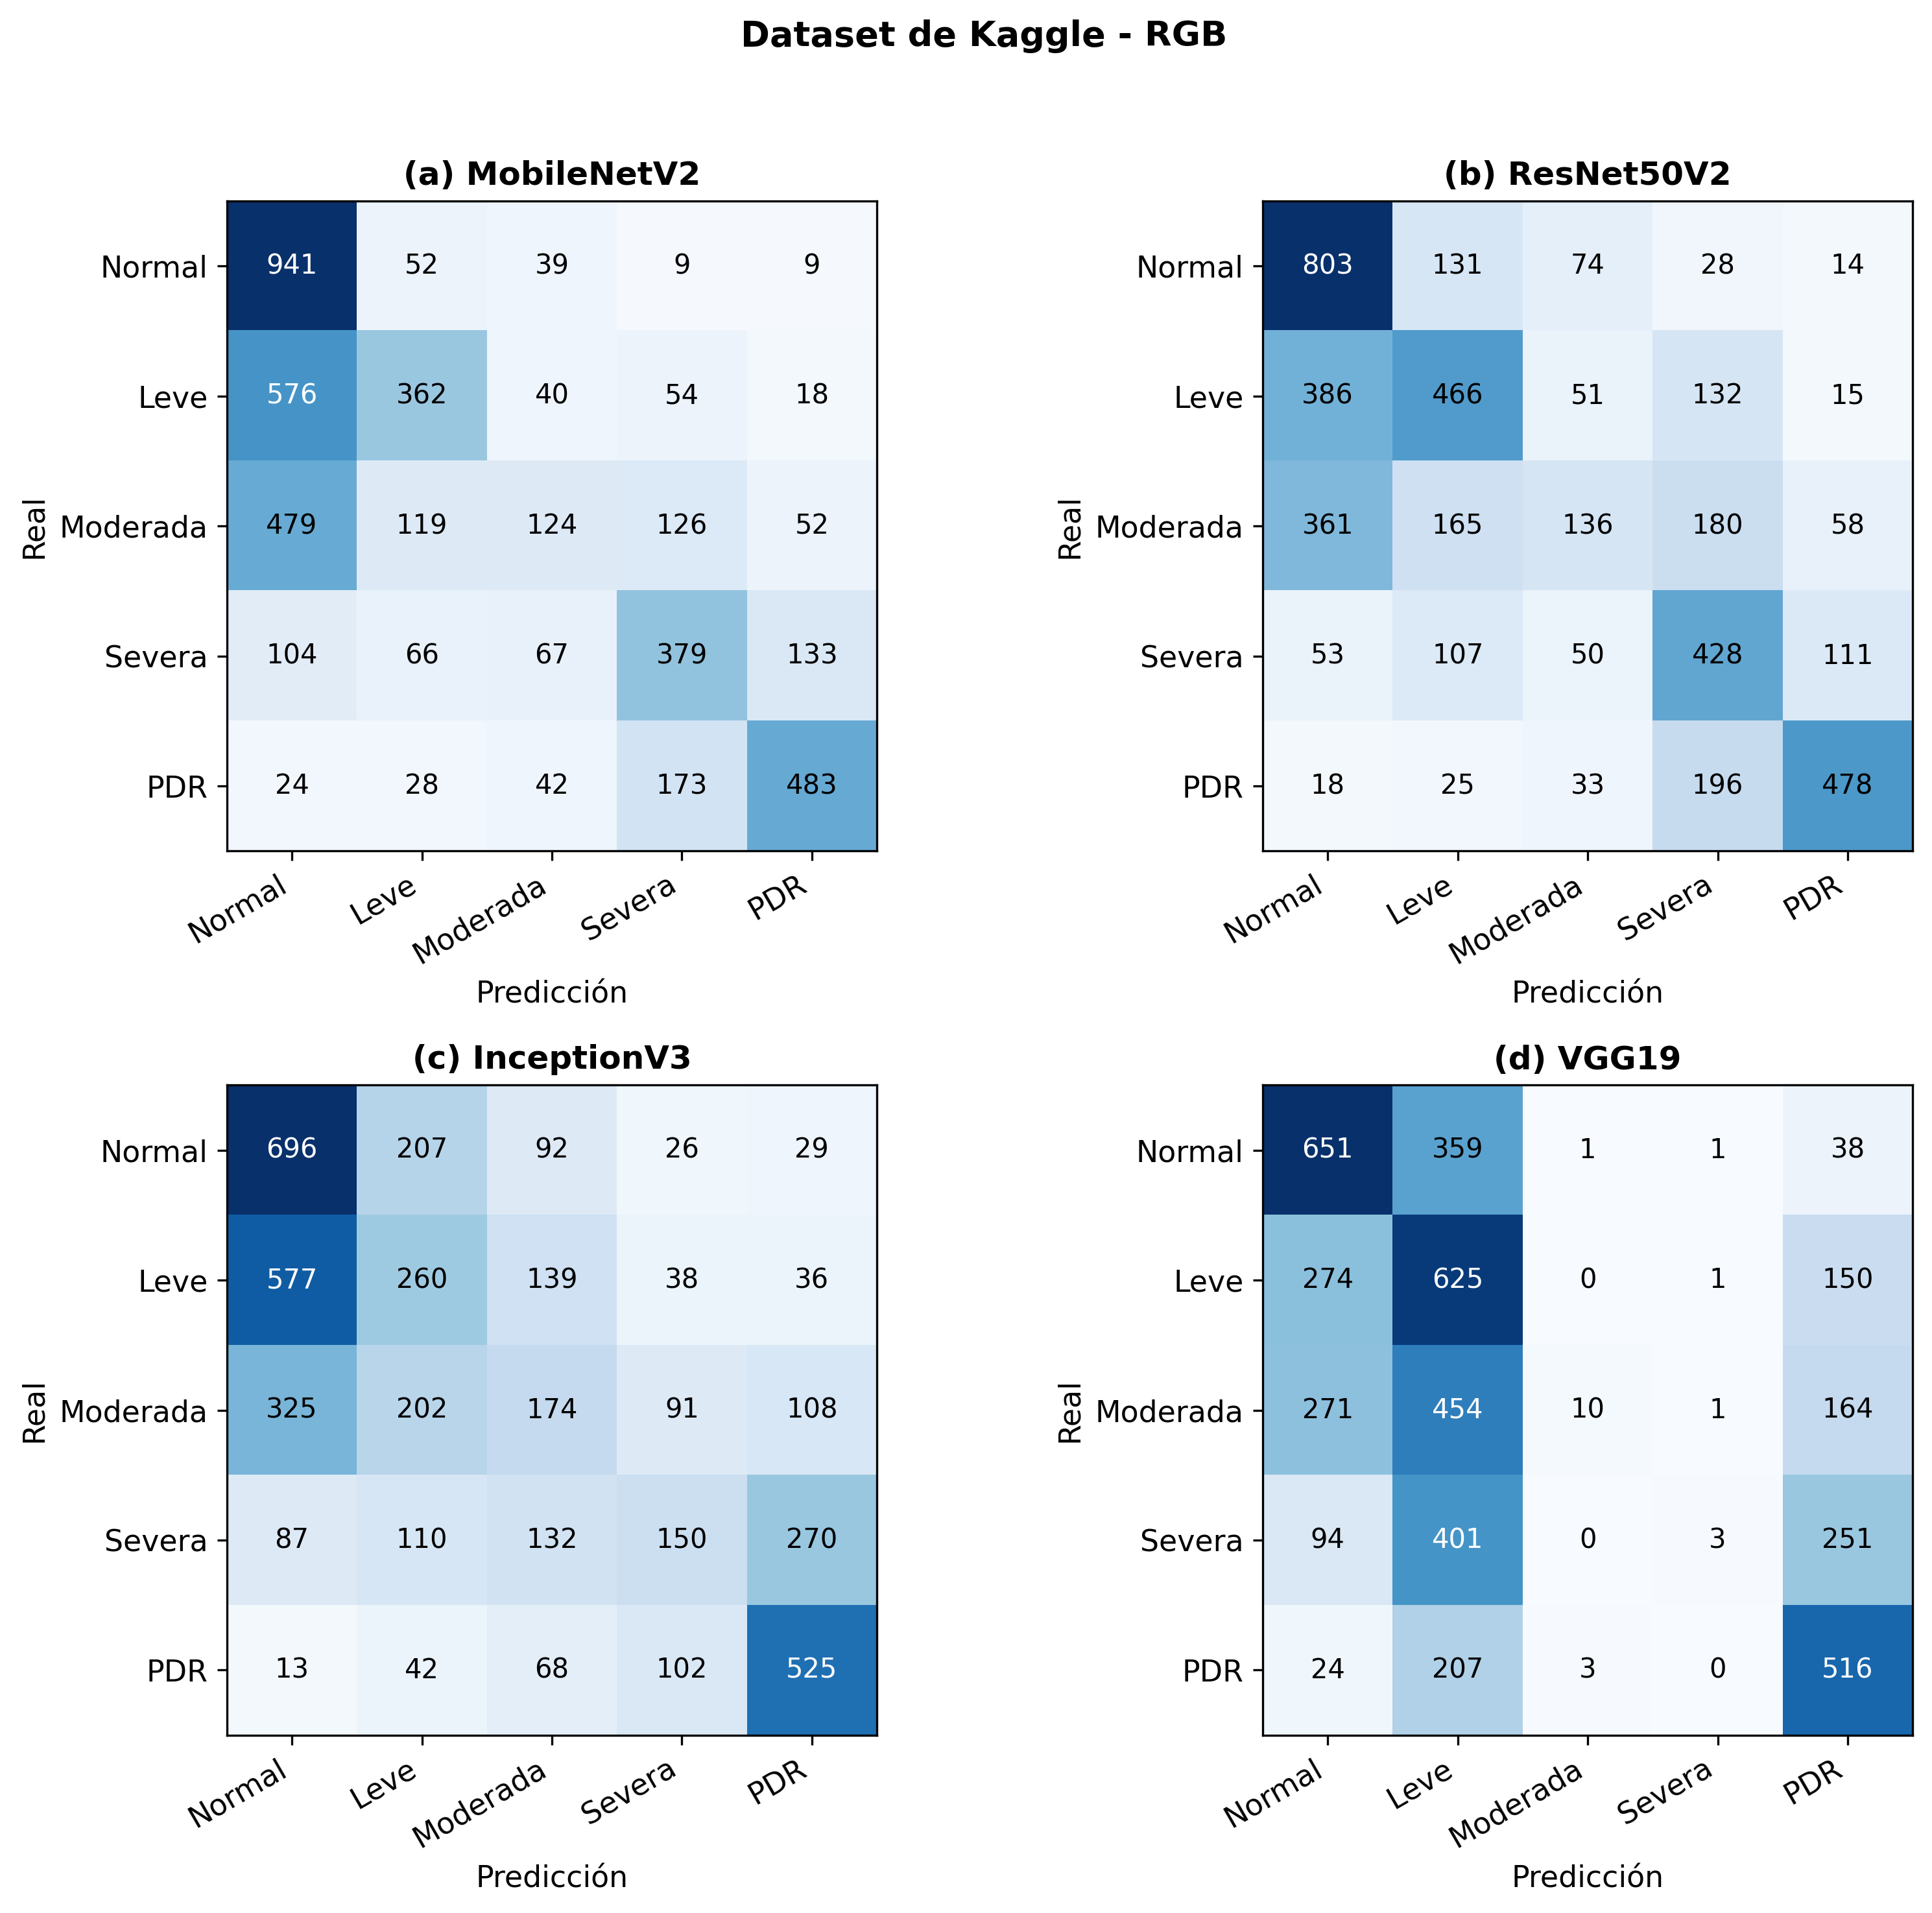
\includegraphics[width=\textwidth]{imágenes/resultados/confusion_multiclase_rgb.png}
	\caption*{\textit{Fuente: Elaboración propia}}
\end{figure}

La Figura~\ref{fig:confusion-multiclase-verde} repite este ejercicio utilizando
únicamente el canal verde como entrada; el lector puede comparar directamente esta
matriz contra la de la Figura~\ref{fig:confusion-multiclase-rgb} para observar el efecto
del canal sobre la distribución de aciertos y errores de cada arquitectura.

\begin{figure}[H]
	\centering
	\caption{Matriz de confusión para la evaluación de cada clasificador multiclase usando el
	dataset de Kaggle canal \textbf{VERDE}}
	\label{fig:confusion-multiclase-verde}
	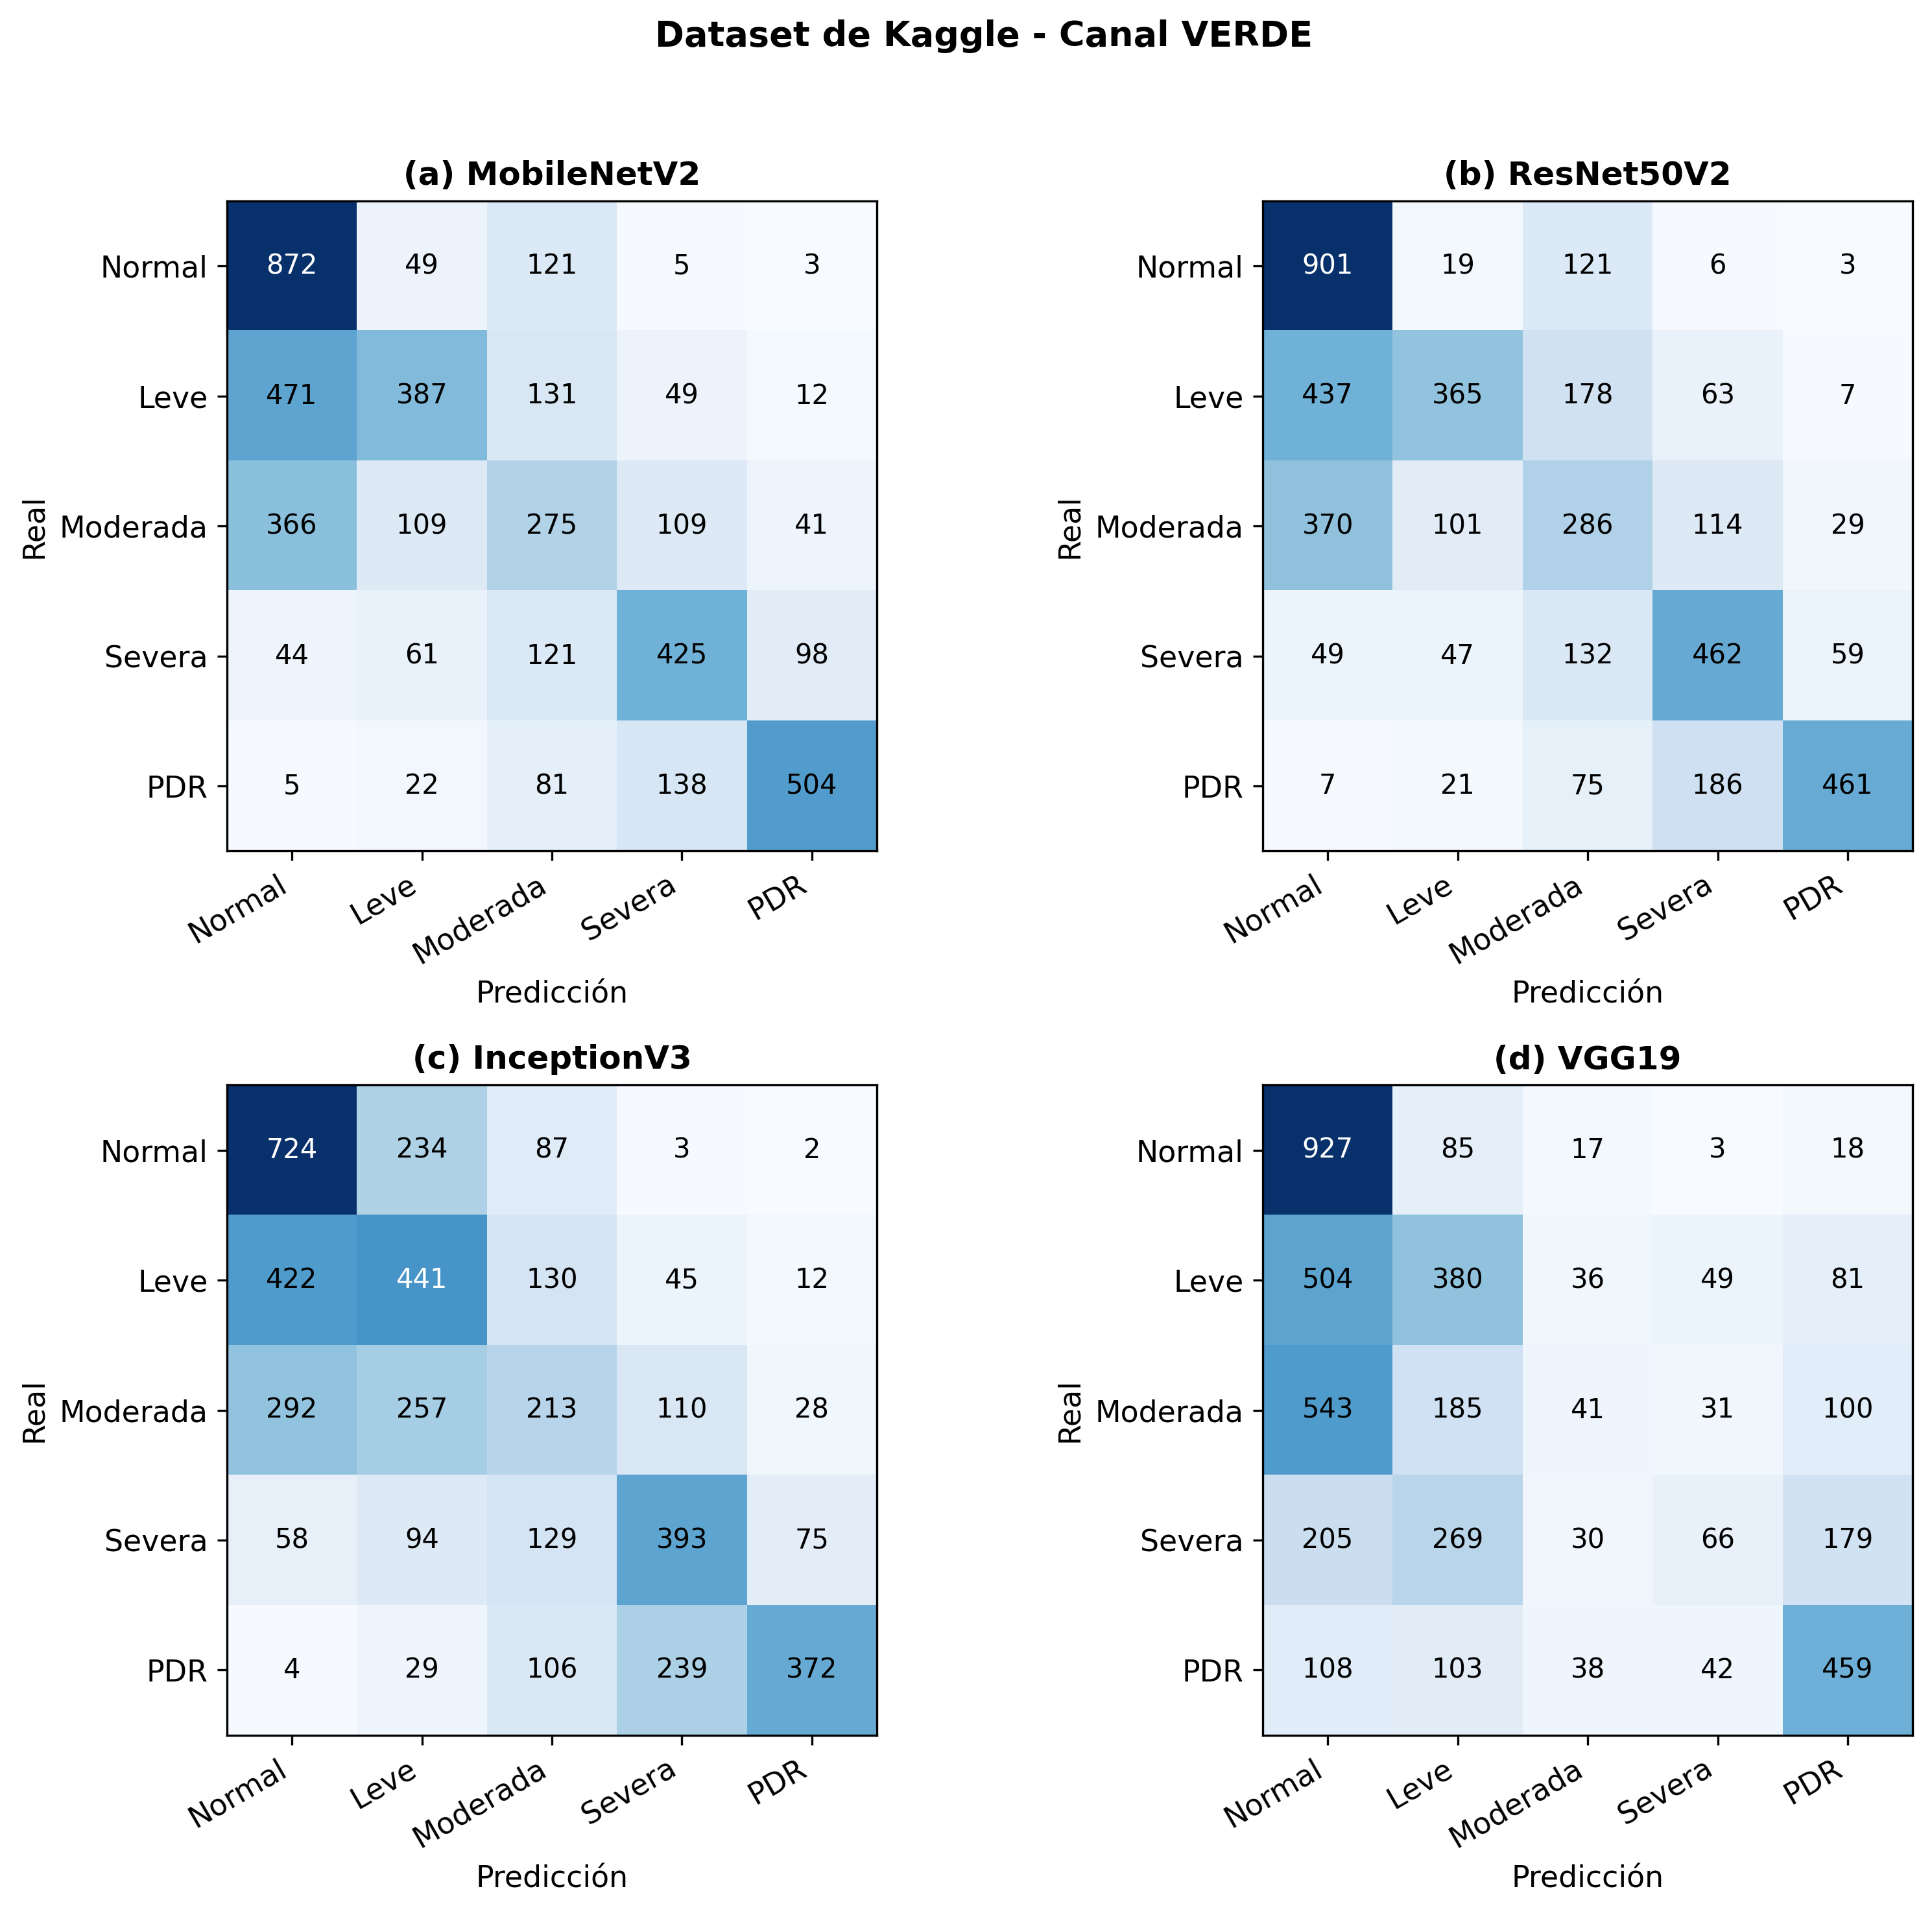
\includegraphics[width=\textwidth]{imágenes/resultados/confusion_multiclase_verde.png}
	\caption*{\textit{Fuente: Elaboración propia}}
\end{figure}

La Figura~\ref{fig:confusion-multiclase-azul} presenta el mismo ejercicio para el canal
azul, uno de los dos canales individuales (junto con el rojo) que obtuvo un desempeño
agregado considerablemente inferior al del canal verde (Sección~
\ref{subsec:analisis-canales}).

\begin{figure}[H]
	\centering
	\caption{Matriz de confusión para la evaluación de cada clasificador multiclase usando el
	dataset de Kaggle canal \textbf{AZUL}}
	\label{fig:confusion-multiclase-azul}
	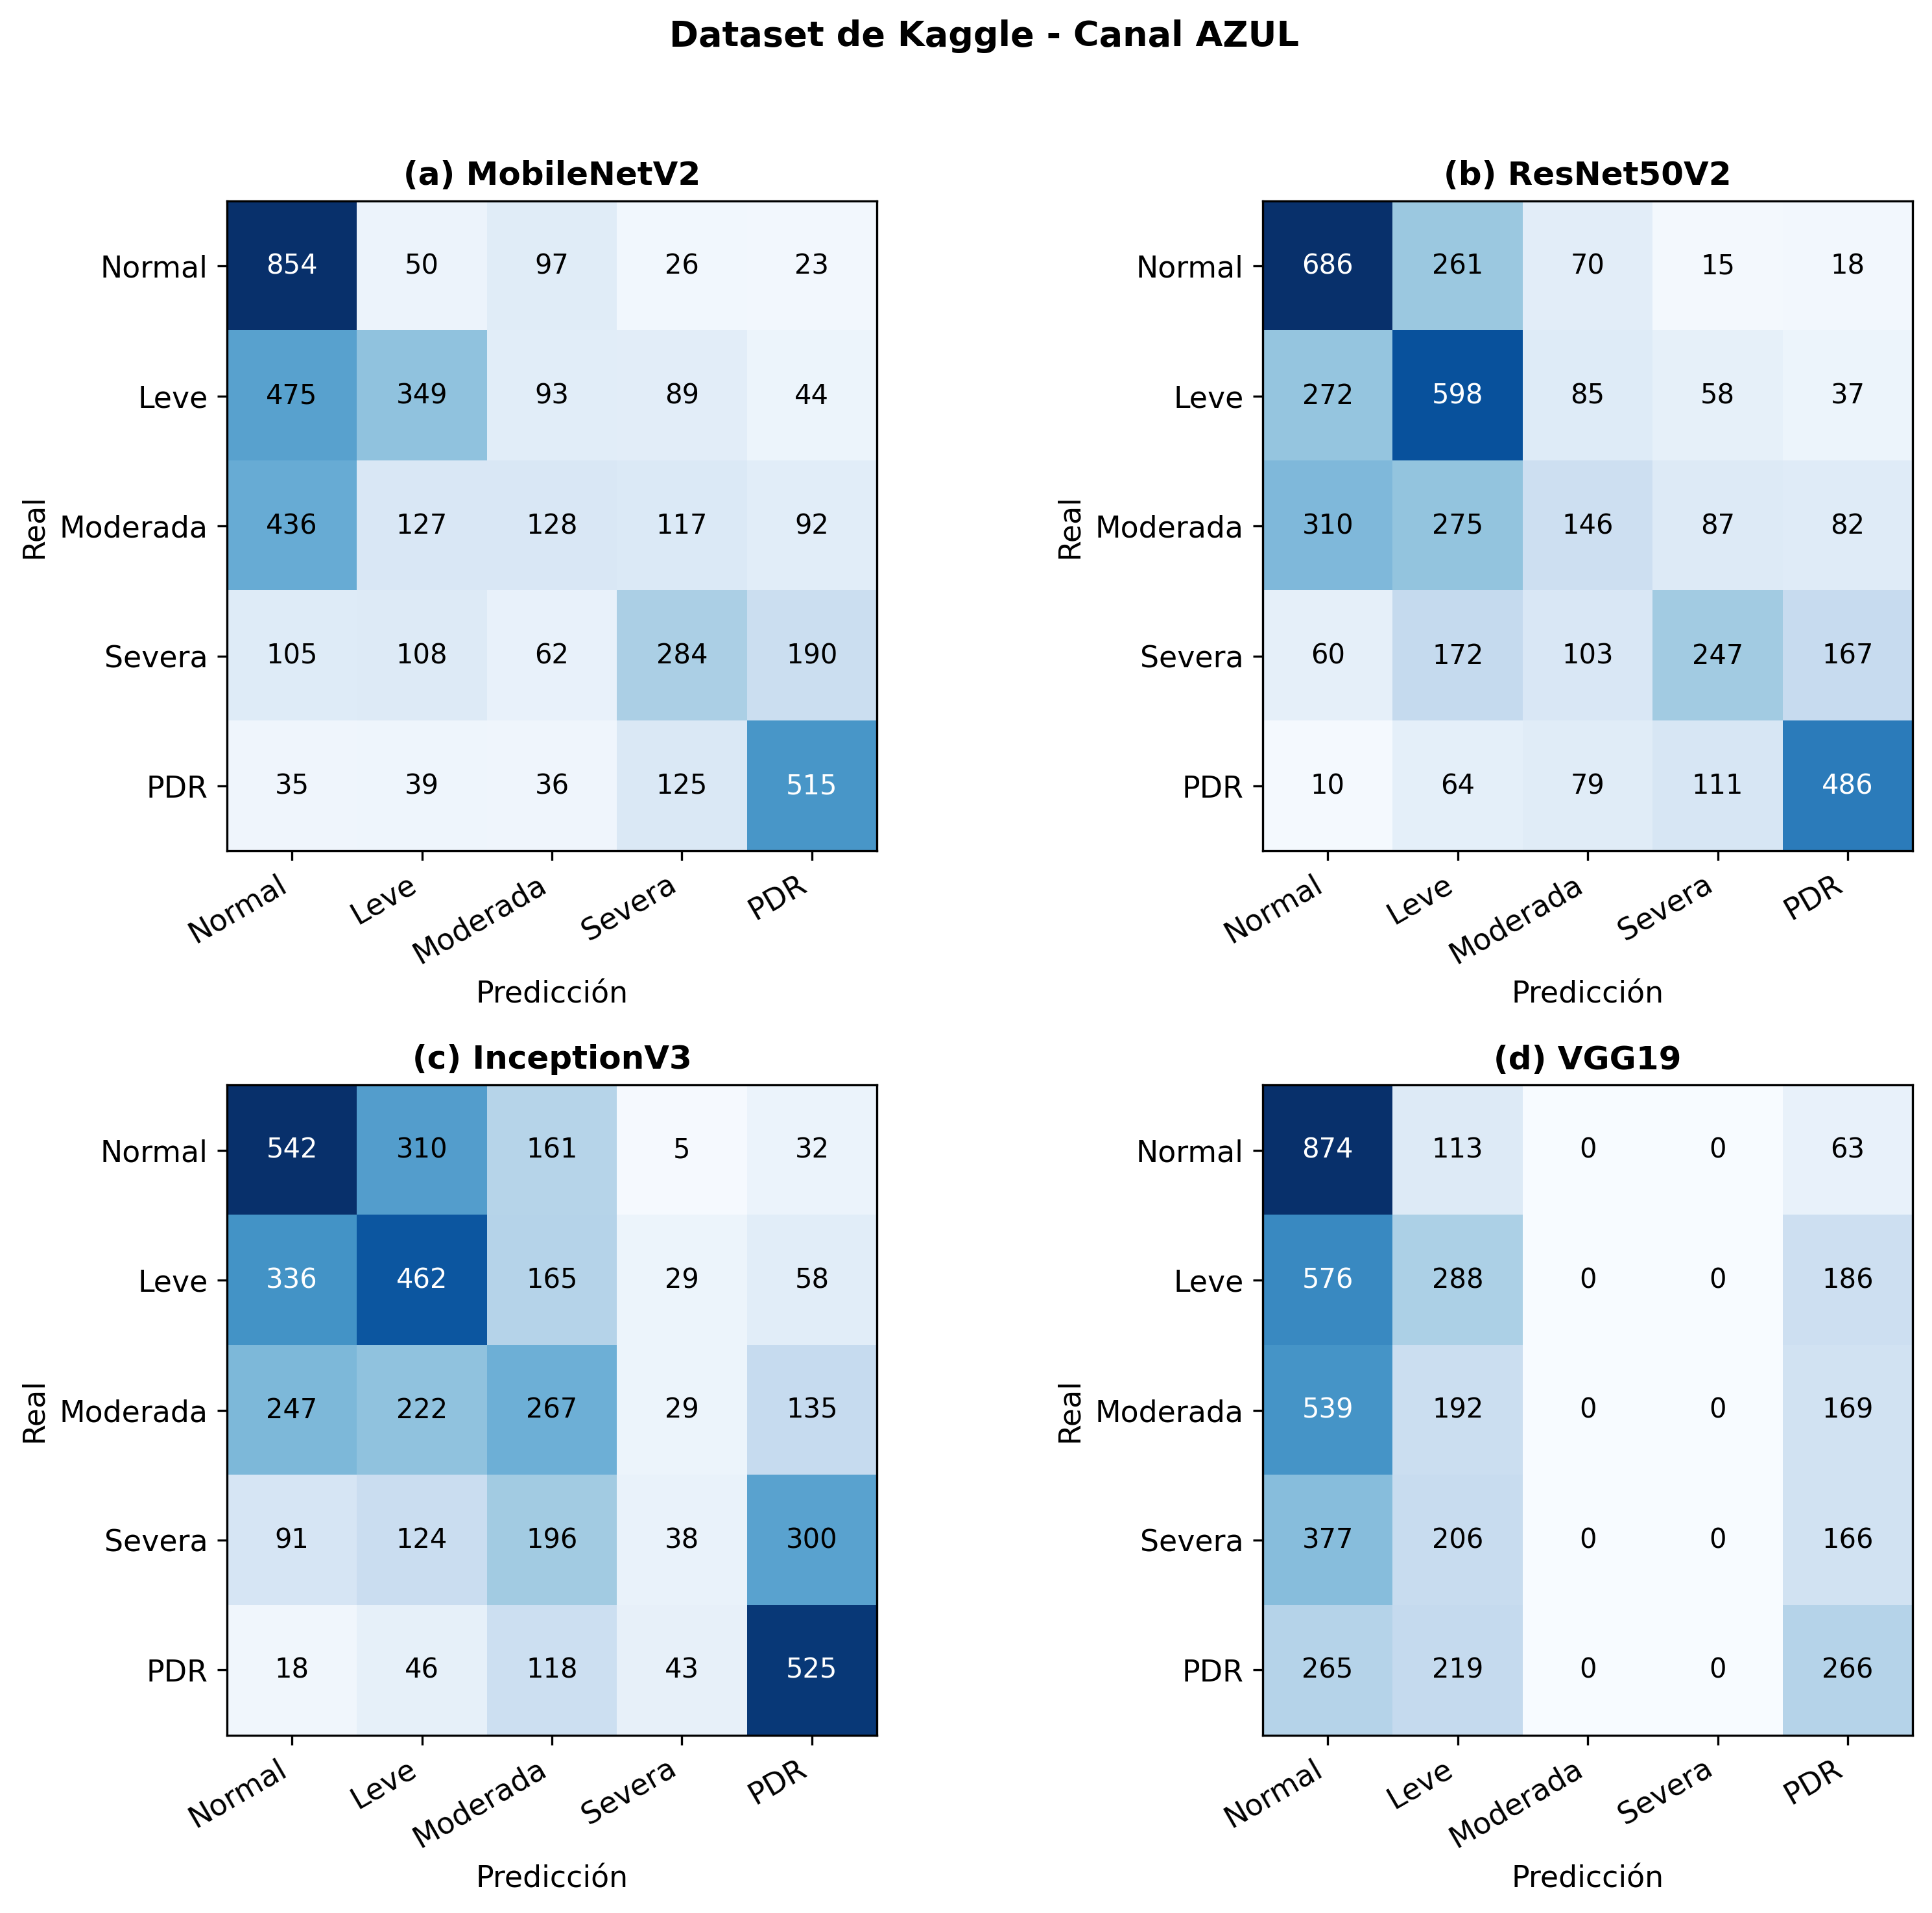
\includegraphics[width=\textwidth]{imágenes/resultados/confusion_multiclase_azul.png}
	\caption*{\textit{Fuente: Elaboración propia}}
\end{figure}

Finalmente, la Figura~\ref{fig:confusion-multiclase-rojo} presenta las matrices de
confusión para el canal rojo, con el cual se completa la comparación de las cuatro
configuraciones de entrada evaluadas.

\begin{figure}[H]
	\centering
	\caption{Matriz de confusión para la evaluación de cada clasificador multiclase usando el
	dataset de Kaggle canal \textbf{ROJO}}
	\label{fig:confusion-multiclase-rojo}
	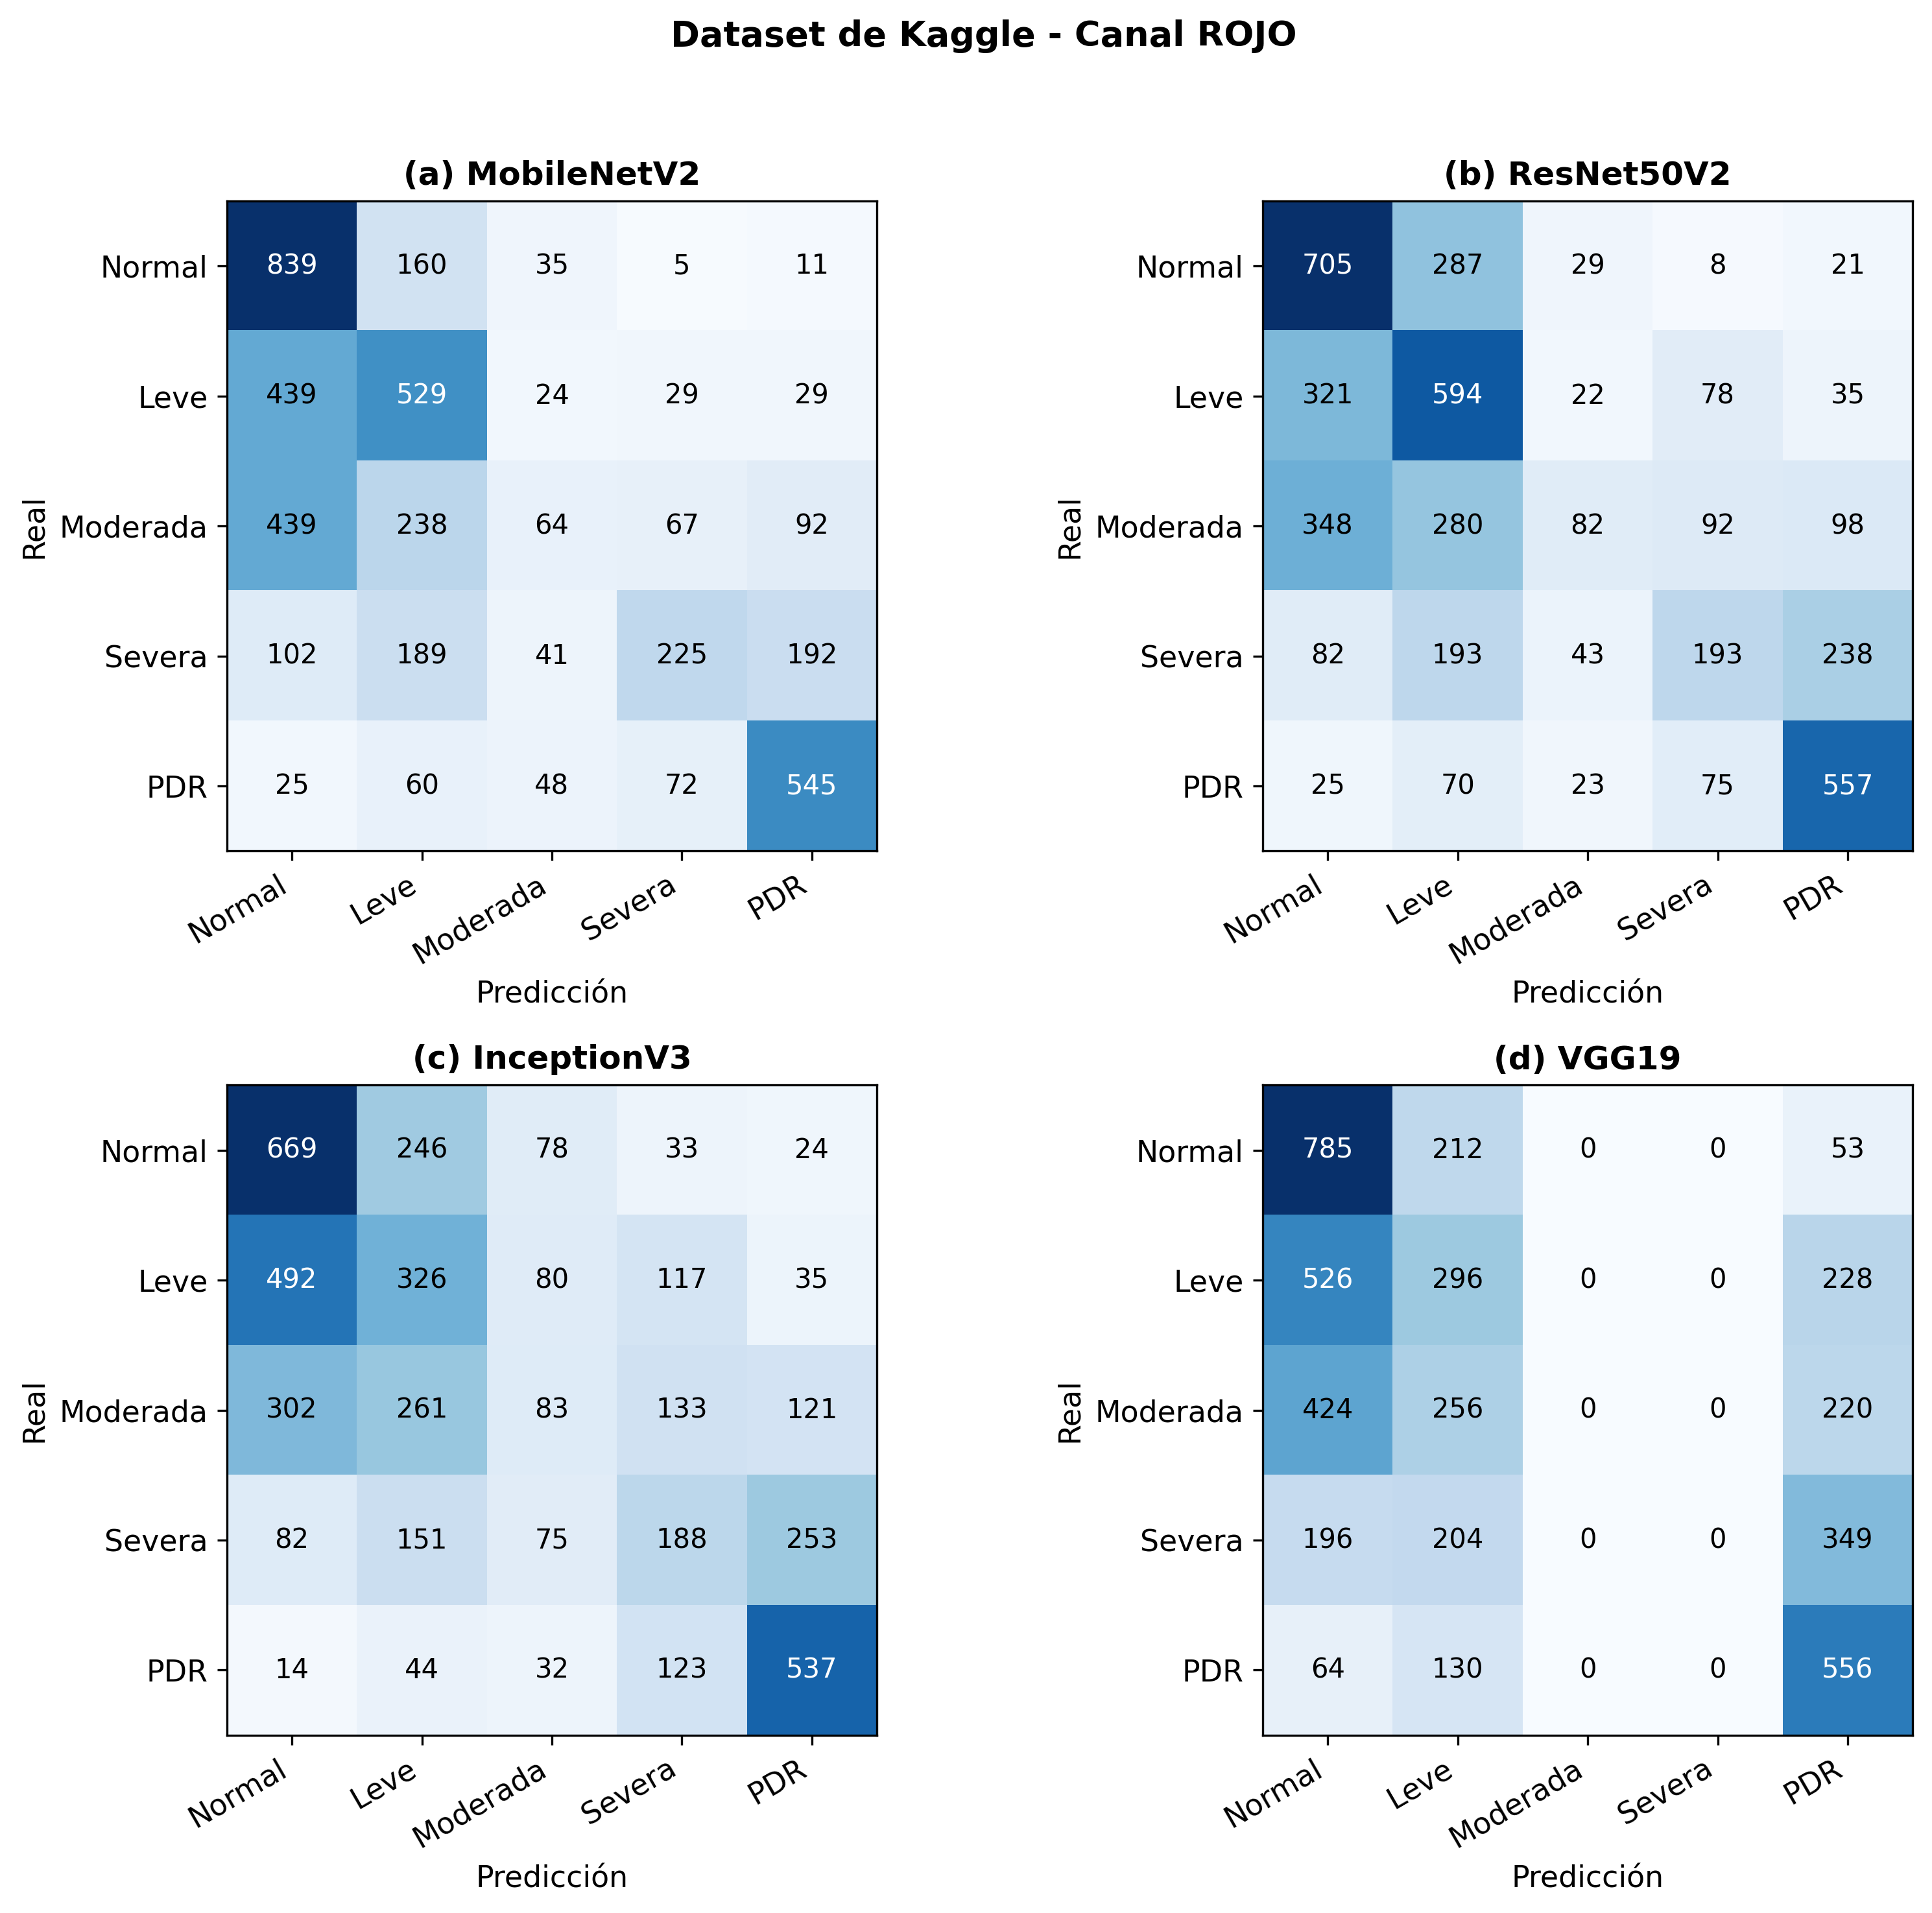
\includegraphics[width=\textwidth]{imágenes/resultados/confusion_multiclase_rojo.png}
	\caption*{\textit{Fuente: Elaboración propia}}
\end{figure}

Para sintetizar estas 16 matrices de confusión en cifras comparables, la
Tabla~\ref{tab:metricas-multiclase-canales} agrega sensibilidad, especificidad,
precisión y F1-score de cada arquitectura para las cuatro configuraciones de entrada; en
ella se observa que MobileNetV2 y ResNet50V2 con el canal verde obtienen el mejor
F1-score (0.54) de toda la comparación, con MobileNetV2 destacándose además por la mayor
sensibilidad (0.65).

\begin{table}[H]
	\centering
	\renewcommand{\arraystretch}{0.8}
	\caption{Desempeño de redes preentrenadas para la clasificación multiclase de
	retinopatía diabética usando todos y cada uno de los canales \textbf{RGB}}
	\label{tab:metricas-multiclase-canales}
	\begin{tabularx}{\textwidth}{l Y Y Y r}
		\toprule
		\multicolumn{5}{c}{RGB} \\
		\midrule
		Red Pre-entrenada  & Sensibilidad & Especificidad &  Precisión & F1-score \\
		\midrule
		MobileNetV2    & 0.55 & 0.87 & 0.52 & 0.50 \\
		ResNet50V2 & 0.51 & 0.88 & 0.51 & 0.49 \\
		InceptionV3& 0.39 & 0.85 & 0.40 & 0.39 \\
		VGG19& 0.38 & 0.85 & 0.50 & 0.31\\
		\multicolumn{5}{c}{Canal rojo} \\
		\midrule
		Red Pre-entrenada  & Sensibilidad & Especificidad &  Precisión & F1-score \\
		\midrule
		MobileNetV2    & 0.48 & 0.87 & 0.48 & 0.45 \\
		ResNet50V2 & 0.47 & 0.87 & 0.46 & 0.43 \\
		InceptionV3& 0.40 & 0.85 & 0.37 & 0.37 \\
		VGG19& 0.35 & 0.84 & 0.21 & 0.26 \\
		\midrule
		\multicolumn{5}{c}{Canal Verde} \\
		\midrule
		Red Pre-entrenada  & Sensibilidad & Especificidad &  Precisión & F1-score \\
		\midrule
		\textbf{MobileNetV2}    & \textbf{0.65} & \textbf{0.89} & \textbf{0.53} & \textbf{0.54} \\
		ResNet50V2 & 0.58 & 0.89 & 0.55 & 0.54 \\
		InceptionV3 & 0.48 & 0.87 & 0.50 & 0.47 \\
		VGG19 & 0.38 & 0.85 & 0.40 & 0.34 \\
		\midrule
		\multicolumn{5}{c}{Canal Azul} \\
		\midrule
		Red Pre-entrenada  & Sensibilidad & Especificidad &  Precisión & F1-score \\
		\midrule
		MobileNetV2    & 0.47 & 0.87 & 0.46 & 0.44 \\
		ResNet50V2 & 0.48 & 0.87 & 0.46 & 0.46 \\
		InceptionV3& 0.41 & 0.85 & 0.38 & 0.38 \\
		VGG19& 0.29 & 0.82 & 0.19 & 0.22 \\
		\bottomrule
	\end{tabularx}
	\caption*{\textit{Fuente: Elaboración propia}}
\end{table}

Más allá de identificar cuál configuración obtiene el mayor F1-score puntual, es posible
cuantificar la magnitud de la ventaja del canal verde promediando su efecto en las cuatro
arquitecturas. La Tabla~\ref{tab:mejora-canal-verde} muestra que, en promedio, el canal
verde mejora el F1-score en +0.05 puntos (+11.8\%) respecto a la imagen RGB completa, en
+0.095 puntos (+25.2\%) respecto al canal rojo y en +0.0975 puntos (+26.0\%) respecto al
canal azul. La ventaja es consistente en las cuatro arquitecturas evaluadas: incluso en el
caso menos favorable (MobileNetV2 frente a RGB) el canal verde aporta una mejora de
+8.0\%, mientras que en el caso más favorable (VGG19 frente al canal azul) la mejora
relativa alcanza +54.5\%, aunque este último valor debe interpretarse con cautela porque
la configuración VGG19-azul corresponde a un modelo colapsado que nunca predice las clases
Moderada ni Severa (Figura~\ref{fig:confusion-multiclase-azul}, panel d). En términos de
sensibilidad el patrón se repite: el canal verde promedia 0.52 frente a 0.46 de RGB
(+14.2\%), 0.43 de rojo (+22.9\%) y 0.41 de azul (+26.7\%).

\begin{table}[H]
	\centering
	\caption{Mejora del canal verde frente a las demás configuraciones de entrada en
	F1-score (clasificación multiclase)}
	\label{tab:mejora-canal-verde}
	\begin{tabularx}{\textwidth}{l Y Y Y}
		\toprule
		Red Pre-entrenada & $\Delta$F1 vs. RGB & $\Delta$F1 vs. Rojo & $\Delta$F1 vs. Azul \\
		\midrule
		MobileNetV2 & +0.04 (+8.0\%) & +0.09 (+20.0\%) & +0.10 (+22.7\%) \\
		ResNet50V2  & +0.05 (+10.2\%) & +0.11 (+25.6\%) & +0.08 (+17.4\%) \\
		InceptionV3 & +0.08 (+20.5\%) & +0.10 (+27.0\%) & +0.09 (+23.7\%) \\
		VGG19       & +0.03 (+9.7\%) & +0.08 (+30.8\%) & +0.12 (+54.5\%) \\
		\midrule
		\textbf{Promedio} & \textbf{+0.05 (+11.8\%)} & \textbf{+0.095 (+25.2\%)} & \textbf{+0.0975 (+26.0\%)} \\
		\bottomrule
	\end{tabularx}
	\caption*{\textit{Fuente: Elaboración propia. El promedio se calcula como la diferencia
	entre las medias de F1-score de las cuatro arquitecturas para cada configuración.}}
\end{table}

Esta ventaja no se distribuye de manera uniforme entre las cinco clases, sino que se
concentra en las categorías definidas clínicamente por una mayor densidad de lesiones
hemorrágicas y microvasculares. Según los criterios de severidad de la escala ICDR, la
retinopatía severa (RD3) se distingue de la moderada por un incremento sustancial en el
conteo de hemorragias intrarretinianas, anomalías microvasculares intrarretinianas (IRMA)
y arrosariamiento venoso, lesiones que, de acuerdo con el principio de absorción
diferencial de la hemoglobina citado anteriormente \myfootcite{pao2020bichannel}, son
precisamente las que el canal verde realza. Calculando la sensibilidad por clase a partir
de las matrices de confusión ya presentadas (Figuras~\ref{fig:confusion-multiclase-rgb} a
\ref{fig:confusion-multiclase-rojo}), se observa que para la clase Severa el canal verde
eleva la sensibilidad de MobileNetV2 de 0.51 (RGB) a 0.57, frente a apenas 0.30 con el
canal rojo (+90\% relativo) y 0.38 con el canal azul (+50\% relativo); en ResNet50V2 el
efecto es aún más marcado, con una sensibilidad de 0.62 para el canal verde frente a 0.57
(RGB), 0.26 (rojo, +139\% relativo) y 0.33 (azul, +88\% relativo). Este patrón respalda la
hipótesis de que la ventaja del canal verde no es un artefacto estadístico, sino que
responde a una mejor representación de las lesiones que definen clínicamente la severidad
de la enfermedad.

Cabe señalar que esta ventaja no se extiende de forma uniforme a la clase PDR (RD4): en
ambas arquitecturas el canal rojo iguala o supera al verde en la sensibilidad de esta
categoría (0.73 frente a 0.67 en MobileNetV2 y 0.74 frente a 0.61 en ResNet50V2), lo cual
sugiere
que en la etapa proliferativa la vasculatura de neoformación, capturada con mayor
contraste por el canal rojo, aporta información complementaria que el canal verde no
logra representar igual de bien. En conjunto, estos resultados matizan la ventaja del
canal verde: es consistente y cuantificable en el desempeño agregado y particularmente
pronunciada en la clase Severa, pero no representa una superioridad absoluta en todas las
categorías clínicas.


